\chapter{3-D Hand Pose Estimation from Depth Sensors}
\label{chap/hand}

\section{Introduction}
%Articulated hand pose estimation has been a longstanding challenge in computer vision. 
%It is essential to various applications including user human-computer interaction, graphics and activity analysis.
%It shares a lot of similarities with the popular 3-D body pose estimation. 
Articulated hand pose estimation shares a lot of similarities with the popular 3-D body pose estimation. 
Both tasks aim to recognise the configuration of an articulated subject with a high degree of freedom. 
%They also require domain knowledge, \eg kinematics \cite{LaGorce2011} or actions \cite{Yu2013}, in order to infer articulated poses from limited input data. 
While latest depth sensor technologies has enabled body pose estimation in real-time \cite{Baak2011, Shotton2011, Girshick2011, Sun2012}, hand pose estimation still remains unresolved.
Despite their similarities, proven approaches in body pose estimation cannot be repurposed directly to hand articulations, due to the unique challenges of the task:   \\
\textbf{(1) Occlusions and viewpoint changes.} Self occlusions are prevalent in hand articulations. %The complex anatomy of human hand provides at least 26 degrees of freedom. 
Compared with limbs in body pose, fingers perform more sophisticated articulations. 
%In addition, d
Different from body poses which are usually upright and frontal \cite{Eichner2012}, different viewpoints can render different depth images despite the same hand articulation. \\  
\textbf{(2) Noisy hand pose data.} Body poses usually occupy larger and relatively static regions in the depth images. 
Hands, however, are often captured in a lower resolution.
%, which lead to more noisy inputs than that of body poses 
As shown in Fig. \ref{fig/hand/intro}, missing parts and quantisation error is common in hand pose data, especially at small, partially occluded parts such as finger tips. 
%Regardless of the object distance, missing values are created when a complete structured light patterns fail to project on the occlusion boundaries. 
Unlike sensor noise and depth errors in \cite{Girshick2011} and \cite{Baak2011}, these artifacts cannot be repaired or smoothed easily. Consequently, a large discrepancy is observed between synthetic and realistic data. 

Moreover, 
%due to noise, occlusions and the inherent complex structure of human hand, 
manually labelled realistic data are extremely costly to obtain. Existing state-of-the-arts resort to synthetic data, \eg \cite{Keskin2012}, or model-based optimisation, \eg \cite{LaGorce2011, Oikonomidis2012}. Nonetheless, such solutions do not consider the realistic-synthetic discrepancies, their performances are hence affected. Besides, the noisy realistic data make joint detection difficult, whereas in synthetic data joint boundaries are always clean and accurate.

%Whilst handling shape variation is crucial for body pose estimation \cite{Shotton2011}, shape variations of human hands are generally smaller than that of body shape.        

% hand shapes 
\begin{figure}[ht]
\centering 
\subcaptionbox{RGB}[0.22\linewidth]{ \raisebox{-1mm}{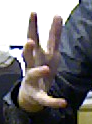
\includegraphics[height=0.27\linewidth]{fig/hand/fig1_rgb.png}} }
\subcaptionbox{Labels}[0.22\linewidth]{ \raisebox{-1mm}{
\includegraphics[height=0.25\linewidth]{fig/hand/fig1_a.png}} }
\subcaptionbox{Synthetic}[0.22\linewidth]{ \raisebox{-1mm}{
\includegraphics[height=0.25\linewidth]{fig/hand/fig1_c.png}} }
\subcaptionbox{Realistic}[0.22\linewidth]{ \raisebox{-1mm}{
\includegraphics[height=0.25\linewidth]{fig/hand/fig1_b.png}} }
\caption{The ring finger is missing due to occlusions in (d), and the little finger is wider than the synthetic image in (c).}
\label{fig/hand/intro}
\end{figure}

In this work, 
addressing the above challenges, 
we present a novel \emph{Semi-supervised Transductive Regression} (\STR) forest
%to address the above challenges
, by learning the relationship between realistic and synthetic data. 
This process is known as \emph{transductive transfer learning} \cite{Pan2010}:   
A transductive model learns from a \emph{source domain}, \eg synthetic data
%, during the training process.
; on the other hand, it applies \emph{knowledge transform} to a different but related \emph{target domain}, \eg realistic data, in the testing stage. 
The \STR\ forest is also semi-supervised, learning the noisy appearances of realistic data from both labelled and unlabelled datapoints. As a result, it benefits from the characteristics of both domain: The \STR\ forest not only captures a wide range of poses from synthetic data, it also achieves promising accuracy in challenging environments by learning from realistic data. 
%In addition to the proposed \STR\ forest, 
In addition, we design an efficient pseudo-kinematic joint refinement algorithm to 
handle occluded and noisy
%deal with the severe occlusion issue in hand
articulations. 
%The proposed method utilises both realistic and synthetically generated training data. 
% a brief decription of the characteristics of our method 

As far as we are aware, the proposed method is the first semi-supervised and transductive articulated hand pose estimation framework.  
The main contribution of our work is threefold:\\ 
\textbf{(1) Realistic-Synthetic fusion:} Considering the issue of noisy inputs, we proposed the first transductive learning algorithm for 3-D hand pose estimation that captures the characteristics of both realistic and synthetic data.\\
%realistic and synthetic data, improving robustness and pose coverage simultaneously. \\
\textbf{(2) Semi-supervised learning:} The proposed learning algorithm utilises both labelled and unlabelled data, improving estimation accuracy while keeping a low labelling cost.  \\
\textbf{(3) Data-driven pseudo-kinematics:} The limitation of traditional Hough forest\cite{Gall2009} against occlusions is improved by learning a data-driven pseudo-kinematic algorithm.


\section{Related Work}

% different shape --- apperance based 
\begin{figure}[ht]
	\hspace{-4mm}
	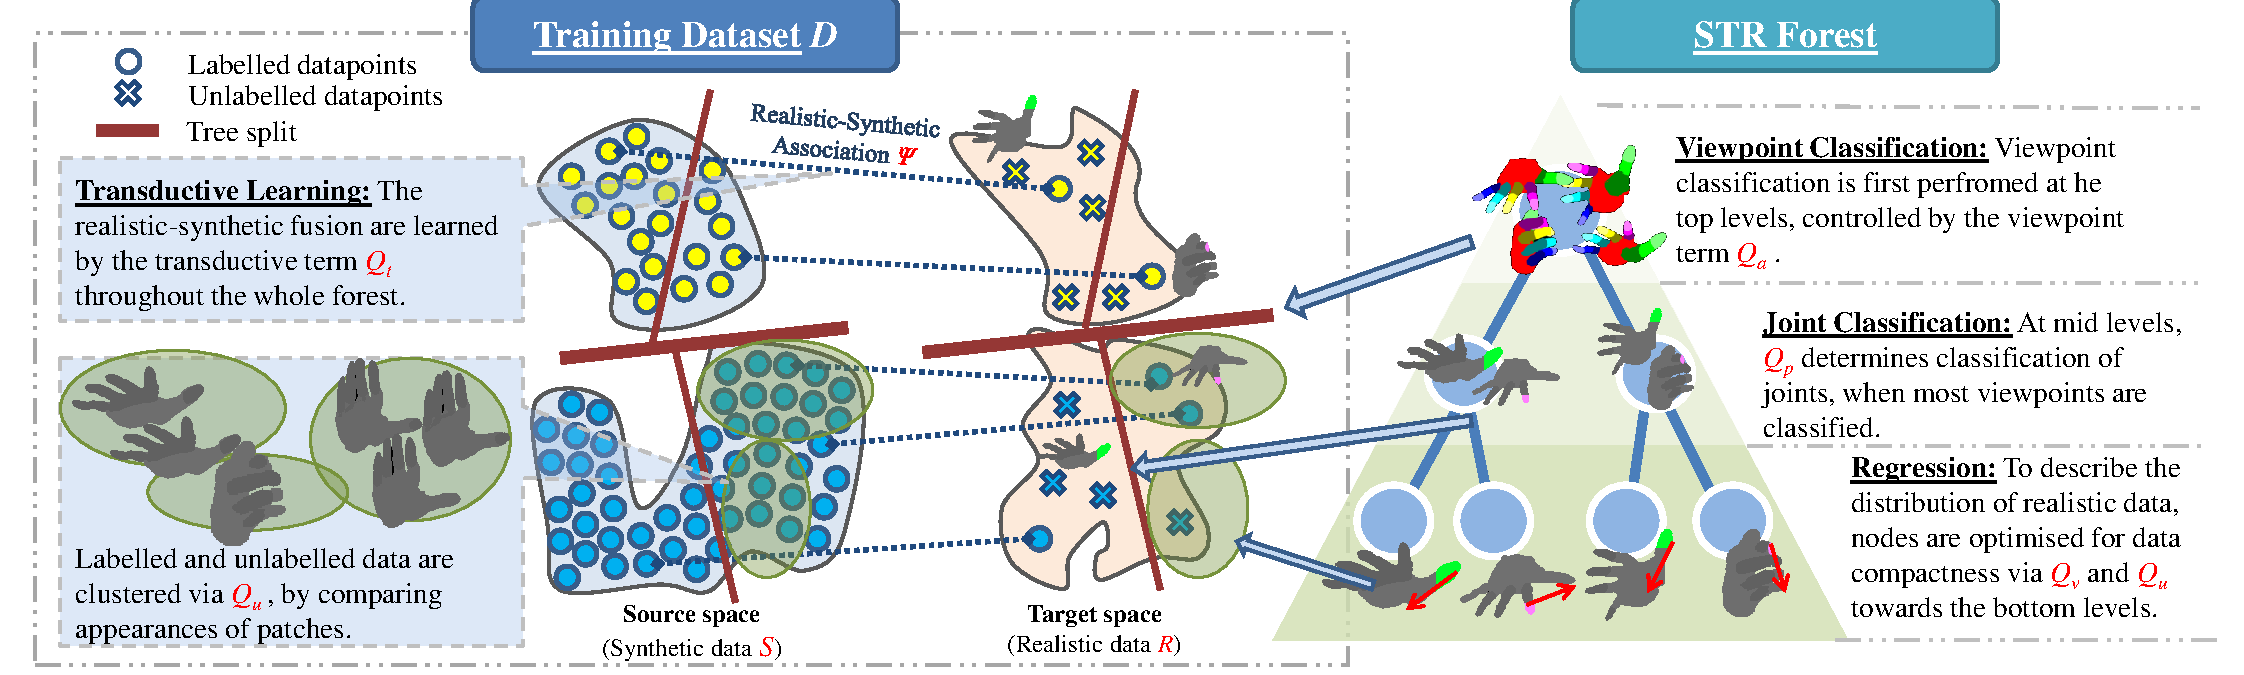
\includegraphics[width=1.03\linewidth]{fig/hand/fig2.pdf}
	\caption{The proposed \STR\ learning model.}
	\label{fig/hand/concept}
\end{figure}

\noindent\textbf{Hand pose estimation} Earlier approaches for articulated hand pose estimation are diversified, such as coloured markers \cite{Chua2002}, probabilistic line matching \cite{Athitsos2003}, multi-camera network \cite{Guan2006} and Bayesian filter with Chamfer matching \cite{Stenger2006}. 
%For example, Chua \etal \cite{Chua2002} recognises hand poses from colored markers on hand to analyse hand articulations. Athitsos \etal \cite{Athitsos2003} estimates articulated hand and viewpoint from a database using probabilistic line matching. Pose ambiguities of hand poses are resolved using multiple cameras in \cite{Guan2006}. Stenger \etal \cite{Stenger2006} infer hand poses using a Bayesian filter based on Chamfer matching. 
We refer the reader to \cite{Erol2007} for a detailed survey of earlier hand pose estimation algorithms. 

\emph{Model-based tracking} methods are popular among recent state-of-the-arts. Hypotheses are generated from a visual model, \eg a 3-D hand mesh. Hand poses are tracked by fitting the hypotheses to the test data. For example, De La Gorce \etal \cite{LaGorce2011} use a hand mesh with detailed simulated texture and lighting. Hamer \etal \cite{Hamer2009} address strong occlusions using local trackers at separate hand segments. Ballan \etal \cite{Ballan2012} infer finger articulations by detecting salient points.  
Oikonomidis \etal \cite{Oikonomidis2011} estimate hand poses in real-time from RGB-D images using particle swarm optimisation. Model-based approaches inherently handle joint articulations and viewpoint changes. 
However, their performances depend on the previous pose estimations, output poses may drift away from groundtruth when error accumulates over time. 
%When tracking is eventually lost, the incorrect poses cannot be recovered without manual re-initialisation.   
%Most model-based methods do not consider shape variations of hands due to the additional complexity involved \cite{Erol2007}, which jeopardises their accuracies in realistic applications. 

\emph{Discriminative} approaches learn a mapping from visual features to the target parameter space, such as joint labels \cite{Shotton2011} or joint coordinates \cite{Girshick2011}.  
Instead of using a predefined visual model, discriminative methods learn a pose estimator from a labelled training dataset. 
Although discriminative methods have proved successful in real-time body pose estimation from depth sensors \cite{Shotton2011, Girshick2011, Baak2011, Sun2012}, they are less common than model-based approaches with respect to hand pose estimation. 
Recent discriminative algorithms for hand pose estimation include approximate nearest neighbour search \cite{Romero2009, Wang2009} and hierarchical random forests \cite{Keskin2012}. 

Discriminative methods rely heavily on the quality of training data. A large labelled dataset is necessary to model a wide range of poses. 
%The main limitation of discriminative approach is that they rely heavily on training data. The performance of a discriminative pose estimator is determined by its training dataset. 

It is also costly to label sufficient realistic data for training. As a result, existing approaches resort to synthetic data by means of computer graphics \cite{Romero2009, Keskin2012}, which suffer from the realistic-synthetic discrepancies.
On the positive side, discriminative methods are frame-based such that there exists no track drifting issue. 
%In addition, driscriminative methods handle shape variations more efficiently by generating extra synthetic training data with different hand shapes.   

%
%The diversity of recognisable pose is typically determined by the training dataset used.  
%However, it is costly to collect sufficient 
%Since the diversity of recognisable poses is determined by the training dataset used, discriminati .
%
%Bad point 1: very costly to gather training data. 
%Good point 1: no tracking, frame by frame so no lost tracking 
%Good point 2: shape variation
%
%\emph{Discriminative} methods learn a pose estimator that appearance features extracted from the input data to the output pose parameter space, \ie joint labels. 
%Instead of a hand-designed visual model as in model-based methods, discriminative approaches require labelled dataset to build the pose estimator.  
%
%
%Approaches for articulated hand pose estimation are categorised into \emph{appearance-based} and \emph{model-based} methods. In model-based methods, hypotheses are generated from a visual model, \eg a deformable hand mesh. They are subsequently fitted to the test data via an iterative optimisation framework. For instance, \cite{LaGorce2011} renders synthetic images from a deformable model with detailed texture and lighting.  
%
% some papers on model-based method 
%The main advantage of model-based tracking approach is that they inherently handle both joint articulations and viewpoint changes. 
%However, their iterative optimisation processes are usually computationally expensive. Although near real-time performance has been reported using latest GPU acceleration techniques [FORTH], the model-based algorithms struggles to attain real-time performance in commodaity hardware. 
%In addition, model-based methods do not consider the variations of hand shapes among individuals, affecting their accuracies in realistic situations.
%
%Appearance-based methods learn a pose estimator that maps appearance features extracted from the input data to the output pose parameter space, \ie labels. Instead of using a hand-designed visual model, appearance-based methods require a labelled training dataset to build the pose estimator.
% some papers on appearance based method 
%Since there exists no iterative optimisation is involved in the testing process, appearance-based method is generally faster than model-based method. Run-time performance is the major advantage of appearance-based method over its model-based counterpart. Recently, the bottleneck of feature extraction process is resolved using specialised hardware, \eg [Kinect], achieving real-time performance for practical applications. 
%The main limitation of appearance-based method is that it relies heavily on the training data; A large labelled dataset is often needed to capture a wide range of poses and viewpoints.

\noindent\textbf{Kinematics}   
Inverse kinematics is a standard technique in model-based and tracking approaches for both body \cite{Yao2012, Pons-Moll2011} and hand poses estimation \cite{LaGorce2011, Oikonomidis2012, Stenger2006}. Lacking a deformable visual model, only a few discriminative methods consider the physical properties of hands. For instance, Girshick \etal \cite{Girshick2011} estimates body poses using a simple range heuristic, yet it is inapplicable to hand pose due to self-occlusions.  
Wang \etal \cite{Wang2009} detect joint using a coloured-glove and match them from the groundtruth database. 
%We propose a \emph{data-driven, pseudo-kinematic} method to correct strongly occluded joints from depth images.  
%Distributions of joint locations are precomputed from a large database of synthetic hand articulations. Occluded joint centres are subsequently rectified by matching the visible joints from the corresponding distributions.

\noindent\textbf{Transfer Learning} 
Transductive transfer learning is often employed when training data of the \emph{target domain} are too costly to obtain. It has seen various successful applications \cite{Pan2010}, still it has not been applied in articulated pose estimation. In this work, realistic-synthetic fusion are realised by extending the idea of Bronstein \etal \cite{Bronstein2010} to the proposed \STR\ forest, where the training algorithm preserves the associations between cross-domain data pairs.

\noindent\textbf{Semi-supervised and Regression Forest} Various semi-supervised forest learning algorithms have been proposed. Shotton \etal \cite{Shotton2013} measure data compactness to relate labelled and unlabelled datapoints. Leistner \etal \cite{Leistner2009} design a margin metric to evaluate with unlabelled data. On the other side, regression forest is widely adopted in body pose estimation, \eg \cite{Girshick2011, Sun2012}. The \STR\ forest adaptively combines the aforementioned semi-supervised and regression forest learning techniques in a single frame work, as explained in Section \ref{sec/hand/methodology:strf}.


\section{Methodology}

The concept of \STR\ learning is illustrated in Fig. \ref{fig/hand/concept}. 
For each viewpoint, training data are collected from a partially labelled target domain (realistic depth images) and a fully labelled source domain (synthetic depth images). These domains are explicitly related by establishing associations from the labelled target datapoints to their corresponding source datapoints, as shown in the figure. 

The proposed \STR\ learning algorithm introduces several novel techniques to the traditional Hough/regression forest \cite{Gall2011}. 
Firstly, transductive realistic-synthetic associations are preserved, such that the matched data are passed down to the same node.
Secondly, the distribution of labelled and unlabelled realistic data are modeled jointly in the proposed \STR\ forest using unsupervised learning. 
Lastly, viewpoint changes are handled alongside with hand poses using an adaptive hierarchical classification scheme.
In order to improve estimation performance of occluded and noisy data, we also propose an efficient \emph{data-driven, kinematic-based} method to refine the locations of detected joints.

\subsection{Training datasets}

The training dataset $\totalset = \{\reallset, \realuset, \synset\}$ consists of both realistic data $\realset$ and synthetic data $\synset$. 
A small potion of $\realset$ is labelled, where the labelled and the remaining unlabelled subsets are denoted by $\reallset$ and $\realuset$ respectively. All datapoints in $\synset$ are labelled with groundtruths. The subset of labelled data in $\totalset$ is defined as $\clset = \{\creallset, \csynset\}$.  

All datapoints in $\totalset$ is represented by a local patch, which is randomly sampled from the training depth images. The number of datapoints roughly equals $5\%$ of foreground pixels in the depth images. 

Every datapoint in $\reallset$ or $\synset$ is assigned to a tuple of labels $( \viewlabel, \jointlabel, \votelabel)$. Viewpoint of a patch is represented by the roll, pitch and yaw angles, which are quantised into $\nviewx$, $\nviewy$ and $\nviewz$ steps respectively. The view label $\viewlabel \in \viewlabelset:\mathbb{N}^{3}$ indicates one of the $135$ quantised viewpoints. A datapoint is also given the class label of its closest joint, $\jointlabel \in \{1\dots\njoint\}$, similar to \cite{Shotton2011}.   
Furthermore, every labelled datapoint contains $\njoint$ vote vectors $\votelabel \in \mathbb{R}^{3\times16}$ from the patch's centroid to the 3-D locations of all $\njoint$ joints as in \cite{Gall2011}. 

Realistic-synthetic associations are established through matching datapoints in $\reallset$ and $\synset$, according to their 3-D joint locations.  The realistic-synthetic association $\assoc: \reallset,\synset \rightarrow \{1,0\}$ is defined as below:
\begin{equation}
	\assoc(\real \in \reallset, \syn \in \synset) =
		\begin{cases}
			1 \mbox{ when $\real$ matches $\syn$} \\
			0 \mbox{ otherwise}
		\end{cases}
	\label{eq:association}
\end{equation}

\subsection{\STR\ Forest} 
\label{sec/hand/methodology:strf}
The proposed \STR\ forest performs classification, clustering and regression on both domains in one pose estimator, instead of performing each task in separate forests.    
We grow $\ntree$ decision trees by recursively splitting and passing the current training data to two child nodes. 
The split function of a node is represented by a simple two-pixel test as in Shotton \etal \cite{Shotton2011}. 
%The split function $\splitfunc$ of a node is represented by a simple two-pixel test, as shown in Equation \ref{eq:pixeltest}. 
%\begin{equation}
%	\splitfunc(\patch) = \begin{cases} 
%		\mbox{Left child } & \patch(\textbf{u})-\patch(\textbf{v}) > \tau \\
%		\mbox{Right child } & Otherwise \\
%	\end{cases}
%	\label{eq:pixeltest}
%\end{equation}
%where $\{\textbf{u}$, $\textbf{v}\}$ are two random locations on a datapoint $\patch$; $\tau$ is a random threshold. 
% can delete?  
A group of candidate split functions are generated at each node, the best one is chosen from the candidates by maximising a quality function.   
Instead of using a typical metric such as information gain or label variance \cite{Shotton2013}, we propose two new quality functions.
The quality function is selected at random between $\vpjterm$ and $\tssterm$ for training in Equation \ref{eq:qualityfunction}. 
\begin{equation}
	\begin{cases}
		\vpjterm\!=\!\viewparam\viewterm\!+\!(1\!-\!\viewparam)\classparam\classterm\!+\!(1\!-\!\viewparam)(1\!-\!\classparam)\regterm \\ 
		\tssterm\!=\!\pairterm^{\tssparam}\usterm 
	\end{cases}
	\label{eq:qualityfunction}
\end{equation}
where $\vpjterm$ is a hybrid quality function for learning classification-regression decision trees, and $\tssterm$ enables transductive and semi-supervised learning. 
Given the training data $\ctotalset = \{\creallset, \crealuset, \csynset\}$, the quality functions are defined as below.   

\noindent\textbf{Viewpoint classification term $\viewterm$:} Traditional \emph{information gain} is used to evaluate the classification performance of all the viewpoint labels $\viewlabel$ in dataset $\clset$ \cite{Breiman2001}. Since this term is applied on the top of the hierarchy, a large amount of training samples needs to be evaluated. Inspired by \cite{Girshick2011}, reservoir sampling is employed to avoid memory restriction and speed up training.\\ 
% Note: although I look less rigorous I omitted the arguments in the quality terms, in order to save space
%\begin{equation}
%	\viewterm = 
%	\entropy_{\viewlabel}(\clset) - 
%	\frac{|\clset_{l}|}{|\clset|} \entropy_{\viewlabel}(\clset_{l}) -  
%	\frac{|\clset_{r}|}{|\clset|} \entropy_{\viewlabel}(\clset_{r}). 
%\end{equation}
%where $\entropy_{\viewlabel}(\cdot)$ is the information entropy of viewpoint labels \cite{Breiman2001}. 
%where $\clset_{l}$ and $\clset_{r}$ are the training data that pass down the left and right child nodes respectively. \\ 
\textbf{Patch classification term $\classterm$: } Similar to $\viewterm$, it is the information gain of the joint labels $\jointlabel$ in $\clset$. It measures the performance of classifying individual patch in $\clset$. 
%, by replacing $\entropy_{\viewlabel}(\cdot)$ with $\entropy_{\jointlabel}(\cdot)$:
%\begin{equation}
%	\classterm = 
%	\entropy_{\jointlabel}(\clset) - 
%	\frac{|\clset_{l}|}{|\clset|} \entropy_{\jointlabel}(\clset_{l}) -  
%	\frac{|\clset_{r}|}{|\clset|} \entropy_{\jointlabel}(\clset_{r}). 
%	\label{eq:classterm}
%\end{equation}\\
Thus, $\viewterm$ and $\classterm$ optimises the decision trees by \emph{classifying} $\clset$ their viewpoints and joint labels. \\
\textbf{Regression term $\regterm$:} This term learns the \emph{regression} aspect of the decision trees by measuring the compactness of vote vectors. Given the set of vote vectors $\votelabelset(\clset)$ in $\clset$, regression term $\regterm$ is defined as:
\begin{equation}
	%\begin{split}
	\regterm = \left[ 1 + 
	\frac{|\clset_{lc}|}{|\clset|} \trvar(\votelabelset(\clset_{lc})) +  
\frac{|\clset_{rc}|}{|\clset|} \trvar(\votelabelset(\clset_{rc})) \right]^{-1}
	%\votelabelset(\clset) & = \{ \votelabel_{\patch}|\forall \patch \in \clset \}.
	%\end{split}
	\label{eq:regterm}
\end{equation}
where $\clset_{lc}$ and $\clset_{rc}$ are the training data that pass down the left and right child nodes respectively, and $\trvar(\cdot) = \mathrm{trace}(\mathrm{var}(\cdot))$ is the trace of variance operator in \cite{Gall2011}. 
$\regterm$ increases with compactness in vote space and converges to $1$ when all votes in a node are identical. \\ 
\textbf{Unsupervised term $\usterm$:} The appearances the target domain, \ie realistic data, are modeled in an \emph{unsupervised} manner. 
Assuming appearances and poses are correlated under the same viewpoint, $\usterm$ evaluates the appearance similarities of all realistic patches $\realset$ within a node:    
\begin{equation}
	\usterm = \left[ 1 + 
	\frac{|\crealset_{lc}|}{|\crealset|} \trvar(\crealset_{lc}) +  
\frac{|\crealset_{rc}|}{|\crealset|} \trvar(\crealset_{rc}) \right]^{-1}.  
	\label{eq:usterm}
\end{equation}
Since the realistic dataset is sparsely labelled, \ie$|\crealuset| \gg |\creallset|$, $\crealuset$ are essential for modeling the target distribution. 
In order to speed up the learning process, $\usterm$ can be approximated by down-sampling the patches in $\crealset$. \\  
\textbf{Transductive term $\pairterm$:} 
%The relationship between the sparse realistic data and dense synthetic data is learned via \emph{transductive learning}. 
Inspired from cross-modality boosting in \cite{Bronstein2010}, 
the \emph{transductive} term $\pairterm$ preserves the cross-domain associations $\assoc$ as the training data pass down the trees: 
%the cross-domain associations are preserved as the training data pass down the trees: 
\begin{equation}
	\begin{split}
	\pairterm &= 
	\frac{|\{r,s\} \subset \clset_{lc}| +  
	|\{r,s\} \subset \clset_{rc}|}{|\{r,s\} \subset \clset|} \\   
	\forall\ \{r,s\} &\subset \clset \mbox{ where } \assoc(r,s) = 1
	\end{split}
	\label{eq:pairterm}
\end{equation}
The transductive term $\pairterm$ is hence the ratio of preserved association after a split. \\
\textbf{Adaptive switching$\{\viewparam, \classparam, \regparam, \tssparam\}$} 
A decision tree mainly performs classifications at the top levels, its training objective is switched adaptively to regression at the bottom levels (Fig. \ref{fig/hand/concept}). 
%Fig. \ref{fig/hand/concept} illustrates the coarse-to-fine structure of trees in the proposed approach. 
Let $\margin(\cdot)$ be the difference between the highest posterior of a class and the second highest posterior in a node. $\margin_{\viewlabel}(\clset)$ and $\margin_{\jointlabel}(\clset)$ denote the margin measures of viewpoint labels $\viewlabel$ and joint labels $\jointlabel$ in $\clset$. They measure the purity of a node with respect to viewpoint and patch label.   
\begin{equation}
	\hspace{-3mm}
	\begin{array}{l@{}r}
	\viewparam  = 
	\begin{cases}
		1\mbox{ if } \margin_{\viewlabel}(\clset) < t_{\viewparam} \\
		0\mbox{ otherwise }
	\end{cases} & 
	\classparam = 
	\begin{cases}
		1\mbox{ if } \margin_{\jointlabel}(\clset) < t_{\classparam} \\
		0\mbox{ otherwise}
	\end{cases}
		\end{array}
	\label{eq:switchparam}
\end{equation}
where $t_{\viewparam}$ and $t_{\classparam}$ are predefined thresholds that determine the structure of the output decision trees. The parameter $\tssparam$ controls the relative importance of transductive term $\pairterm$ to unsupervised term $\usterm$.  

%\begin{algorithm}
%	\label{alg:transductive}
%	\KwData{Training dataset $\totalset = \{ \reallset, \realuset, \synset \}$ }
%	\KwResult{A classification-regression tree trained on both domains that can test on realistic domain.}
%	Let = $\{\reallset, \realuset, \synset \} = \{\creallset, \crealuset, \csynset\}$\\
%	Randomly generate a set of tests $\splitfuncset = \{\mathbf{u}, \mathbf{v}, \tau\}$ \\ 
%	Randomly select one of the following quality functions in Equation \ref{eq:qualityfunction} for evaluating $\splitfuncset$.\\ 
%	\ForEach{$\splitfunc \in \splitfuncset$}{
%		Partition $\ctotalset$ into two subsets $\ctotalset_l$ and $\ctotalset_r$ by $\splitfuncc$\\
%		Measure the partition with selected quality function.
%	}
%	Choose the optimal $\splitfunc$ and partition by maximizing selected measurement: 
%		$ \splitfuncc = \argmax_{\splitfunc}\qterm(\splitfunc) $\\ 
%		%In the optimal partition, if any association $\assoc(r,s)$ is broken, a copy of $\{r,s\}$ is made so that $\{r,s\} \in X_l$ and $\{r,s\} \in X_r$.\\
%	Recursively perform step 1-7 for $\ctotalset_l$ and $\ctotalset_r$ until $|\ctotalset|<n$, where $n$ is the minimum samples of nodes.
%	\caption{Tranductive training with RF}
%\end{algorithm}


\subsection{Data-driven Kinematic Joint Refinement}

Since the proposed \STR\ forest considers joint as independent detection targets, it lacks structural information to recover poorly detected joints when they are occluded or missing from the depth image. 
Without having an explicit hand model as in most model-based tracking methods, we designed a data-driven, kinematic-based method to refine joint locations from the \STR\ forest. 
A large hand pose database $\ksynset$ is generated, such that $|\ksynset| \gg |\synset|$, in order to obtain the maximum pose coverage. The pose database $\ksynset$ is generated using the same hand model as in the synthetic dataset $\synset$, but $\ksynset$ contains only the joint coordinates. 

The procedures for computing the data-driven kinematic model $\GMM$ is described in Algorithm \ref{alg:kinematic}. $\GMM$ contains viewpoint-specific distributions of joint locations represented as a $\ngmm$-part \emph{Gaussian mixture models (GMM)}. 
%The joint refinement algorithm is described in testing as described below. 

\begin{algorithm}
	\KwData{A joint dataset $\ksynset \subset \mathbb{R}^{3\times16}$ that contains synthetic joint locations, where $|\ksynset| \gg |\synset|$. } 
	\KwResult{A set of viewpoint-dependent distributions $\GMM = \{\GMM_{\mathbf{i}}| \forall \mathbf{i} \in \viewlabelset \}$ of global poses.}
	Split $\ksynset$ with respect to viewpoint label $\viewlabelset$, such that $\ksynset = \{ \ksynset_{1} \dots \ksynset_{\nview} \}$\\
	\ForAll{$\mathbf{i} \in \viewlabelset$}{
		Learn a $\ngmm$-part GMM $\GMM_{i}$ of the dataset $\ksynset_{i}$:
		$\GMM_{\mathbf{i}} = \{\mu_{\mathbf{i}}^{1}\dots\mu_{\mathbf{i}}^{n}\dots\mu_{\mathbf{i}}^{\ngmm};\Sigma_{\mathbf{i}}^{1}\cdots\Sigma_{\mathbf{i}}^{n}\cdots\Sigma_{\mathbf{i}}^{\ngmm}\}$, 
		where $\mu_{\mathbf{i}}^{\onegmm}$ and $\Sigma_{\mathbf{i}}^{\onegmm}$ denote the mean and \emph{diagonal} variance of the $n$-th Gaussian component in $\GMM_{\mathbf{i}}$ of viewpoint $\mathbf{i}$. \\
	}
	\caption{Data-driven Kinematic Models.}
	\label{alg:kinematic}
\end{algorithm}

\subsection{Testing} 
\label{sec/hand/methodology:test}
\noindent\textbf{Joint Classification and Detection. } Given a testing image, patches are extracted densely from the testing depth images. Similar to other decision forests, each patch passes down the \STR\ forest to obtain the viewpoint $\testviewlabel$ and vote vectors $\testvotelabel$. The patch vote for all $16$ joint locations according to $\testvotelabel$.   
%Each patch $\testpatch$ in $\testpatchset$ will vote for all $16$ 3-D joint locations.  

\noindent\textbf{Kinematic Joint Refinement. } 
The objective of kinematic joint refinement is to compute the final joint locations $\testjoint = \{ \testonejoint_{1} \dots \testonejoint_{\joint} \dots \testonejoint_{16} | \forall \testonejoint \in \mathbb{R}^{3}\}. $
Derived from the meanshift technique in \cite{Girshick2011}, the distributions of votes vectors are evaluated as stated below: 
The set of votes received by the $\joint$-th joint is fitted a $2$-part GMM $\testGMM_{\joint} = \{ \hat{\mu}_{\joint}^{1}, \hat{\Sigma}_{\joint}^{1}, \hat{\rho}_{\joint}^{1}, \hat{\mu}_{\joint}^{2}, \hat{\Sigma}_{\joint}^{2}, \hat{\rho}_{\joint}^{2} \}$, where $\hat{\mu}$, $\hat{\Sigma}$, $\hat{\rho}$ denote the mean, variance and weight of the Gaussian components respectively. Fig. \ref{fig/hand/refine} visualises the two Gaussian components obtained from fitting the voting vectors of a joint.  

A strong detection forms one compact cluster of votes, which leads to a high weighting and low variance in one of the Gaussians. 
On the contrary, a weak detection usually contains scattered votes, indicated by separated means with similar weights. 
%As a result, the output joint locations $\testjoint:\mathbb{R}^{3\!\times\!16}$ are evaluated and refined by the followings: 
The $\joint$-th joint is of high-confidence 
%A \emph{high-confidence} joint $\testonejoint_{h}$ is defined 
when the Euclidean distance between $\hat{\mu}_{\joint}^{1}$ and $\hat{\mu}_{\joint}^{2}$ is smaller than a threshold $\testqualthres$. 
For any high-confident $j$-th joint, the output location $\testonejoint_{\joint}$ is the mean of the dominating Gaussian in $\testGMM_{\joint}$.  
\begin{equation}
	\testonejoint_{\joint} = 
	\begin{cases}
		\hat{\mu}_{\joint}^{1} & \mbox{ if } ||\hat{\mu}_{\joint}^{1} - \hat{\mu}_{\joint}^{2}||^2_2 < \testqualthres \mbox{ and } \hat{\rho}_{\joint}^{1} \ge \hat{\rho}_{\joint}^{2} \\  
		\hat{\mu}_{\joint}^{2} & \mbox{ if } ||\hat{\mu}_{\joint}^{1} - \hat{\mu}_{\joint}^{2}||^2_2 < \testqualthres \mbox{ and } \hat{\rho}_{\joint}^{1} < \hat{\rho}_{\joint}^{2} \\  
	\end{cases}
	\label{eq:highconf}
\end{equation}

Subsequently, final locations of all high-confidence joints are determined. The joint refinement process is performed on the other low-confidence joints.   

The nearest neighbour of the set of high-confidence joints are searched from its corresponding joint means $\{\mu_{\testviewlabel}^{1}\dots\mu_{\testviewlabel}^{\ngmm}\}$ in the kinematic model $\GMM_{\testviewlabel}$ using least squares with a direct similarity homography. Only the high-confident joint locations are used in the above nearest neighbour matching; the low-confident joint locations are masked out. 
Given the nearest Gaussian component $\{\mu_{\testviewlabel}^{nn}, \Sigma_{\testviewlabel}^{nn}\}$ of the high-confidence joints, each remaining low-confidence joint $\testonejoint_{\joint}$ are refined: 
\begin{equation}
		\{\tilde{\mu}, \tilde{\Sigma}\} 
		= \argmin{\{\mu, \Sigma\} \in \{\hat{\mu}_{\joint}^{1}, \hat{\Sigma}_{\joint}^{1}\},  \{\hat{\mu}_{2}\, \hat{\Sigma}_{2}\}}  
		||\mu - \mu_{\testviewlabel}^{nn}[\joint]||^2_2
		\label{eq:refine1}
\end{equation}
where $\{\tilde{\mu}, \tilde{\Sigma}\}$ is the Gaussian in $\testGMM_{\joint}$ that is closer to the corresponding $\joint$-th joint location in $\{\mu_{\testviewlabel}^{nn}[\joint]:\mathbb{R}^{3}, \Sigma_{\testviewlabel}^{nn}[\joint]:\mathbb{R}^{3\times3}\}$. The final output of a low-confidence joint $\testonejoint_{l}$ is computed by merging the Gaussians in Equation \ref{eq:refine2}. 
\begin{equation}
	\testonejoint_{\joint} =
	\left(\tilde{\Sigma}^{-1}\!+\!(\Sigma_{\testviewlabel}^{nn}[\joint])^{-1}\right)^{-1}\! \left( \tilde{\Sigma} \mu_{\testviewlabel}^{nn}[\joint]\!+\!\Sigma_{\testviewlabel}^{nn}[\joint]\tilde{\mu}\right) 
	\label{eq:refine2}
\end{equation}
Fig. \ref{fig/hand/refine} illustrates the process of refining a low-confidence joint. The middle
proximal joint is occluded by the index finger as seen in the RGB image; the $2$-part GMM $\testGMM_{\joint}$ is represented by the red crosses (mean) and ellipses (variance). The final output is computed by merging the nearest neighbour obtained from $\GMM$, \ie $\{\mu_{\testviewlabel}^{nn}[\joint], \Sigma_{\testviewlabel}^{nn}[\joint]\}$ (the green Gaussian), and the closer Gaussian in $\testGMM_{\joint}$ (the left red Gaussian).  
The procedures of refining output poses $\testjoint$ are stated in Algorithm \ref{alg:testing}.  

\begin{figure}[ht]
	\centering
	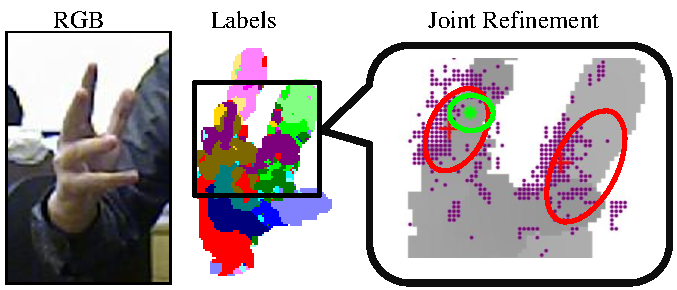
\includegraphics[width=0.8\linewidth]{fig/hand/fig3.pdf}
	\caption{The proposed pseudo-kinematic joint refinement algorithm.}
	\label{fig/hand/refine}
\end{figure}

\begin{algorithm}
	\KwData{Vote vectors obtained from passing down the testing image to the \STR\ forest.}
	\KwResult{The output pose $\testjoint:\mathbb{R}^{3\times16}$.} 
	%Extract patches $\testpatchset$ from depth image $\testimg$ \\ 
	%\ForEach{$\testpatch \in \testpatchset$}{
	%	Compute the viewpoint $\testviewlabel$ and joint $\testjointlabel$. \\ 
	%	Each $\testpatch$ votes at the leaf nodes.
	%}
	\ForEach{ Set of voting vectors for the $\joint$-th joint}{
		%\If {$|\{\testpatch \in \testpatchset| \testjointlabel = j\}| < \testqualthres$}{
		%	Assign the $j$-th joint to the occluded set $\testoccset$. \\
		%}
		Learn a 2-part GMM $\testGMM_{\joint}$ of the voting vectors.\\ 
		\If{$||\hat{\mu}_{\joint}^{1} - \hat{\mu}_{\joint}^{2}||^2_2 < \testqualthres$}{
			The $\joint$-th joint is a high-confidence joint.\\
			Compute the $\joint$-th joint location. (Equation \ref{eq:highconf}) 
		}\Else{
			The $\joint$-th joint is a low-confidence joint.
		}
	}
	Find the Gaussian $\{\mu_{\testviewlabel}^{nn},\Sigma_{\testviewlabel}^{nn}\}$ by finding the nearest neighbour of the high-confidence joints in $\GMM_{\testviewlabel}$.\\ 
	Update the remaining low-confidence joint locations. (Equation \ref{eq:refine1} and \ref{eq:refine2}) \\
	%Assign joint locations in both $\testjointset_{h}$ and $\testjointset_{l}$ to $\testjoint$
	\caption{Pose Refinement} 
	\label{alg:testing}
\end{algorithm}


\section{Experiments}


% How the images are segmented 
% How many training images
% How can the real images be labelled 

\subsection{Evaluation dataset} 

\label{sec/hand/methodology:eval}
Synthetic training data $\synset$ were rendered using an articulated hand model(as shown in Figure~\ref{fig/hand/single}.
Instead of adjusting individual joints, each finger is controlled by a bending parameter, such that only the articulations that can be performed by real hands are considered. 
Hand shapes are mildly randomised when generating the depth images in $\synset$, in order to handle the shape variations in realistic applications. 
Hence, the dataset $\synset$ contains $\nsynperview$ depth images per viewpoint, the size of $\synset$ is $\nsynperview \times 135 = 337.5K$. 

Realistic data $\realset$ were captured using a Asus Xtion depth sensor. There exist about $600$ images per viewpoint, hence the size of $\realset$ is $81K$. Not more than $20\%$ of data in $\realset$ are labelled. The number of labelled sample $|\reallset|$ is around $10K$. Since labels can be reused for the rotationally symmetric images(same yaw and pitch, different roll), only around $1.2K$ of data are hand-labelled.    

For $\reallset$, visible joints were annotated manually using 3-D coordinates but occluded joints are annotated using the $(x,y)$ coordinates only. 
Associations $\assoc$ and the remaining $z$-coordinates in $\reallset$ were computed by matching visible joint locations with $\synset$ using least squares with a direct similarity transform constraint. Consequently, each datapoint in $\reallset$ is paired with its closest match $\patch_{syn} \in \synset$, and its occluded $z$ coordinates were approximated by the corresponding $z$ coordinates of $\patch_{syn}$.
With joint locations as mean, each joint can be model as a 3D truncated Gaussian distribution, where variances can be defined according to hand anatomy. Foreground pixels are clustered into one of these distributions and therefore assigned with labels $\jointlabel$.

For experiments, three different sequences ($A$,$B$ and $C$) are captured and labelled with 450, 1000 and 240 frames respectively. Sequence $A$ has only one viewpoint, $B$ demonstrates viewpoint variation and $C$ has more abrupt changes in both viewpoint and scale. For all experiments, 3 trees are trained with maximum depth varying from 16 to 24, depending on the amount of training data.


% In this work, the training dataset contains $\nsyn$ synthetic depth image and $\nreal$ realistic depth images.  


\subsection{Single View Experiment} 

The proposed approach was evaluated under the frontal view scenario, comparing with the traditional regression forest in \cite{Gall2011} as a baseline. Since there was only one viewpoint in testing sequence $A$,  $\viewterm$ in Equation \ref{eq:qualityfunction} did not affect the experimental results.  
%the difference between our method and the baseline algorithm depends on the performances of joint regression and classification only. 
%thus this experiment only compares the joint classification performance. 
Performances of algorithms are measured by their pixelwise classification accuracy per joint, similar to \cite{Shotton2011}, hence only $\classterm$,$\regterm$, $\pairterm$ and $\usterm$ were utilised in this experiment.    

Fig. \ref{fig/hand/single} shows the classification accuracy plots of the algorithm evaluated in this experiment.  
It demonstrates the strengths of realistic-synthetic fusion and semi-supervised learning. 
Accuracy of baseline method was improved by simply including both domains in training without any algorithmic changes. 

Transductive learning($\pairterm$) substantially improved the accuracy, particularly for the finger joints which were less robust in the baseline algorithms.  
By coupling realistic data with synthetic data, the transductive term $\pairterm$ effectively learns the discrepancies between the domains, which is important in recognising noisy and strongly occluded fingers.
%Transductive learning further helps the decision forest to recognise the intermediate poses between the sparsely labelled realistic data. 
%Weaker joints in transductive learning, \eg joints in little finger tip (L3) and index proximal (I1), are often mislabelled as other more dominating joints.
Some joints are often mislabelled as other more dominating joints after transductive learning, \eg joints in little finger tip (L3) and index proximal (I1). Nevertheless, the semi-supervised framework significantly improved the performances of those joints after transductive learning has applied.  
%Consequently, our semi-supervised framework forms a complement to transductive learning by greatly enhancing the accuracies of these joints. 

\begin{figure}[ht]
	\centering
	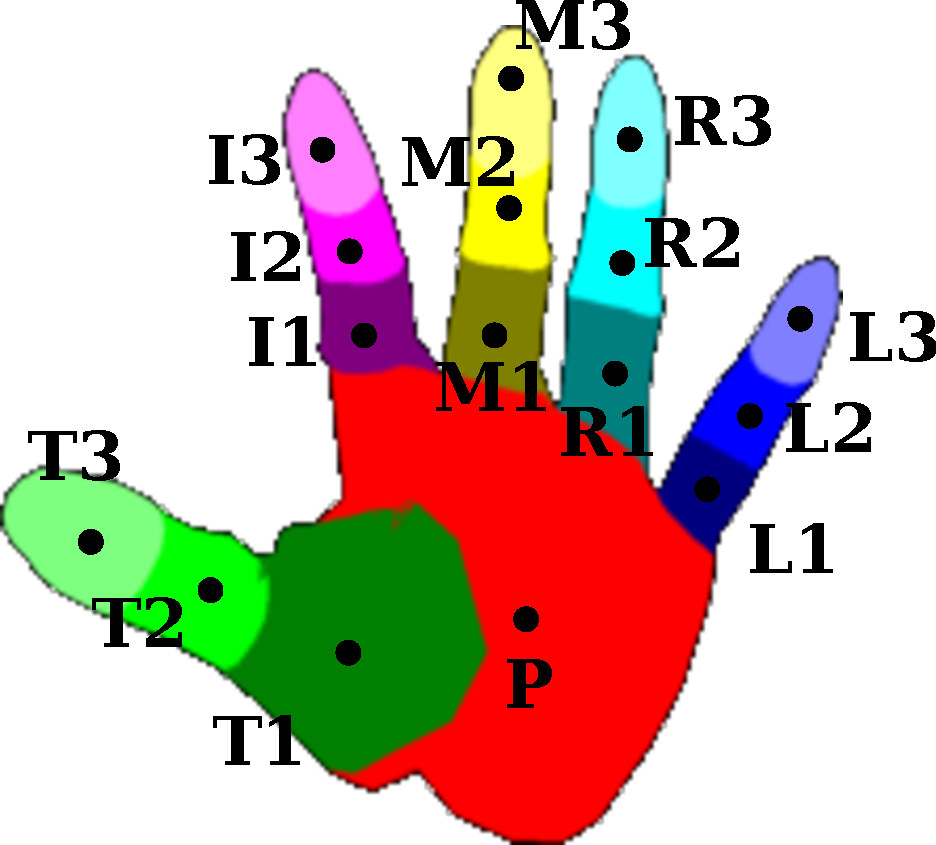
\includegraphics[width=0.22\linewidth]{fig/hand/hand.pdf}
	\caption{Color codes and label names of the 16 hand regions.}
	\label{fig/hand/label}
\end{figure}

\begin{figure}[ht]
	\centering
	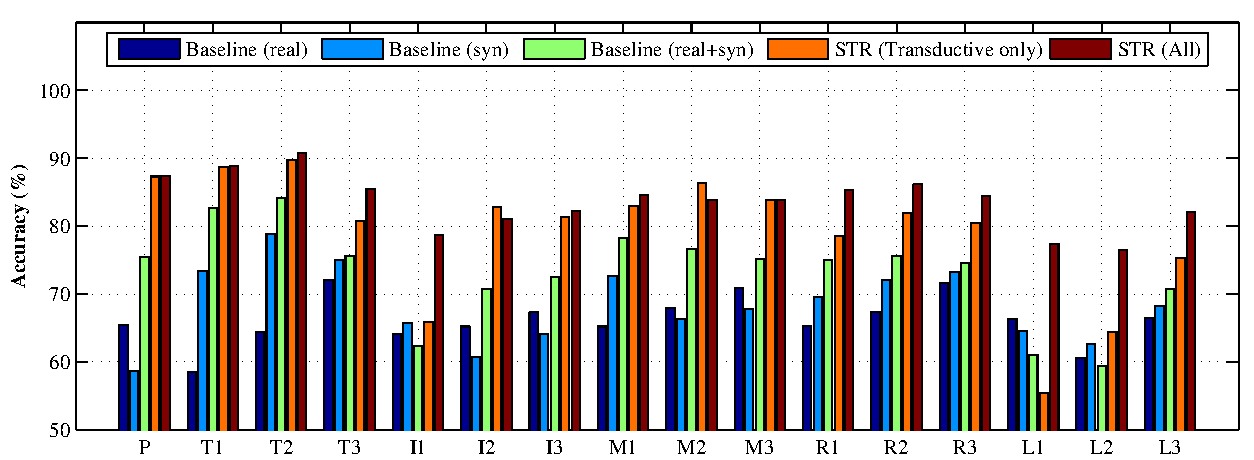
\includegraphics[width=1\linewidth]{fig/hand/singleview.pdf}
	\caption{Joint classification accuracy of the single view sequence.}
	\label{fig/hand/single}
\end{figure}

%\paragraph{Experiment on Data-driven Joint Refinement}
%A fully-labelled, multiview video sequence is recorded to evaluate the overall performances of the approaches.  

\subsection{Multi-view Experiment}  

In the multi-view experiment, the proposed approach was compared with the state-of-the-art by FORTH\cite{Oikonomidis2011} under a challenging multi-view scenario. Quantitative and qualitative evaluations were performed to provide a comprehensive comparison of the methods. 

Hand articulations are estimated from the multi-view testing sequences (sequence $B$ and $C$) by both of the methods. 
%In addition to pose variations in sequence $A$, sequence $B$ contains long and continuous pose and viewpoint changes. 
%Sequence $C$ is particularly challenging as it contains abrupt viewpoint changes and poses with strong occlusions, as visualised in Fig. \ref{fig/hand/experiments:multiview:qual}.
Since FORTH require manual initialisation, the testing sequences used are designed such that they start with the required initialisation pose and position, making a fair comparison.   
Same as \cite{Oikonomidis2011},  
performances of pose estimation were measured by \emph{joint localisation error}.
% necessary? 

\noindent \textbf{Quantitative Results}
Fig. \ref{fig/hand/multiquant} shows the average localisation errors of the two testing sequences. It also shows a representative of error graphs from a stable joint (palm, $P$) and a difficult joint (index finger tip, $I3$). The proposed \STR\ forest, with the data-driven kinematic joint refinement, outperforms FORTH in all three statistics, especially for the finger tip joints that are noisy and frequently occluded. Even though a few large estimation errors are observed, our frame-based approach is able to recover from errors quickly.    

Sequence $C$ further confirm the major advantage of our approach over its tracking-based counterpart---In the first $200$ frames, with kinematic joint refinement, \STR\ forest approach performs just slightly better than FORTH. However, localisation errors in FORTH accumulate after an abrupt change and have not been recovered since then. As model-based tracking approaches rely on previous results to optimise the current hypothesis iteratively, estimation errors amass over time. On the other hand, frame-based discriminative approaches consider each frame as an independent input, enabling fast error recovery at the expense of a smooth and continuous output. 

The proposed joint refinement scheme increases the joint estimation accuracy in general, as shown in Fig. \ref{fig/hand/multiquant}. 
Some of the large classification errors, \eg Fig. \ref{fig/hand/multiquantc}, are fixed after applying joint refinement. It implies that the joint refinement process not only improves the accuracy of joint, but also avoids incorrect detections by validating the output of \STR\ forest with kinematic constraints.

\noindent \textbf{Qualitative Analysis} 
The experimental results are also visualised in Fig. \ref{fig/hand/multiqual} for qualitative evaluation. 
Fig.~\ref{fig/hand/multiqual}a and b show the pose estimation results from different view points.    
Fig.~\ref{fig/hand/multiqual}c shows a frame at the beginning of test sequence $B$, both FORTH and our method obtains accurate hand articulations. Nonetheless, the performance of FORTH declines rapidly in the middle of the sequence when its tracking is lost and failed to recognise Fig.~\ref{fig/hand/multiqual} d, yet our approach still gives correct results. 

Our efficient \STR\ forest also achieves promising run-time performance, it estimates hand poses at about $25$FPS on an Intel I7 PC without GPU acceleration, whilst the FORTH algorithm runs at $6$FPS on the same hardware configuration plus NVidia GT 640. 


%\begin{figure}[ht]
%	\centering
%	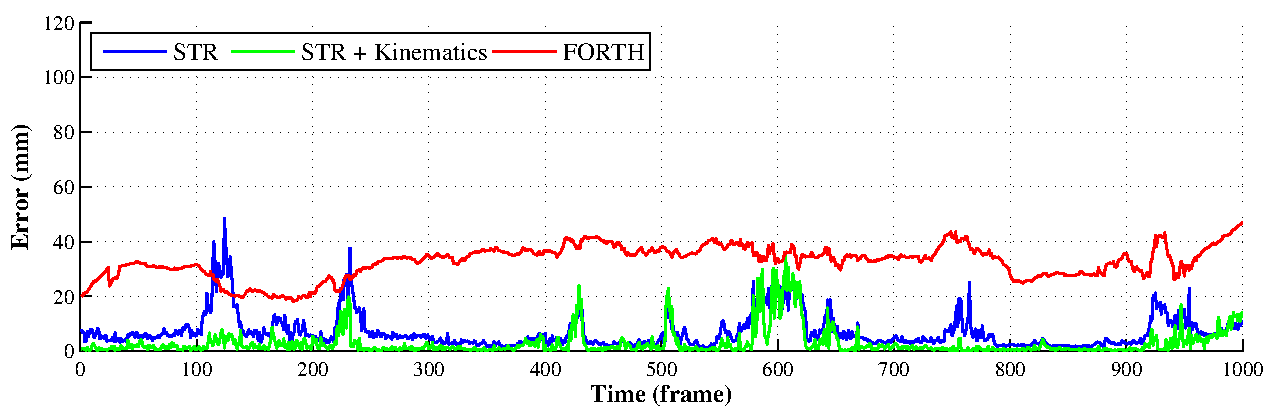
\includegraphics[width=0.33\linewidth]{fig/hand/sq1_avg.pdf}  
%	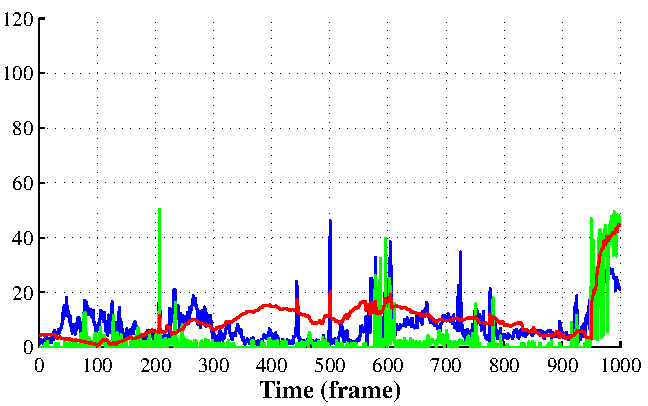
\includegraphics[width=0.31\linewidth]{fig/hand/sq1_palm.pdf} 
%	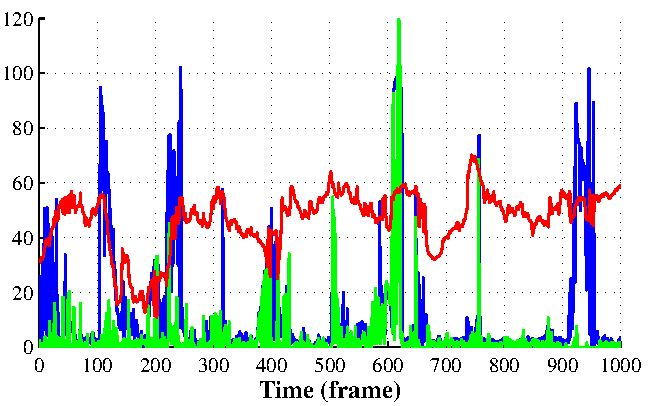
\includegraphics[width=0.31\linewidth]{fig/hand/sq1_tip.pdf} \\
%	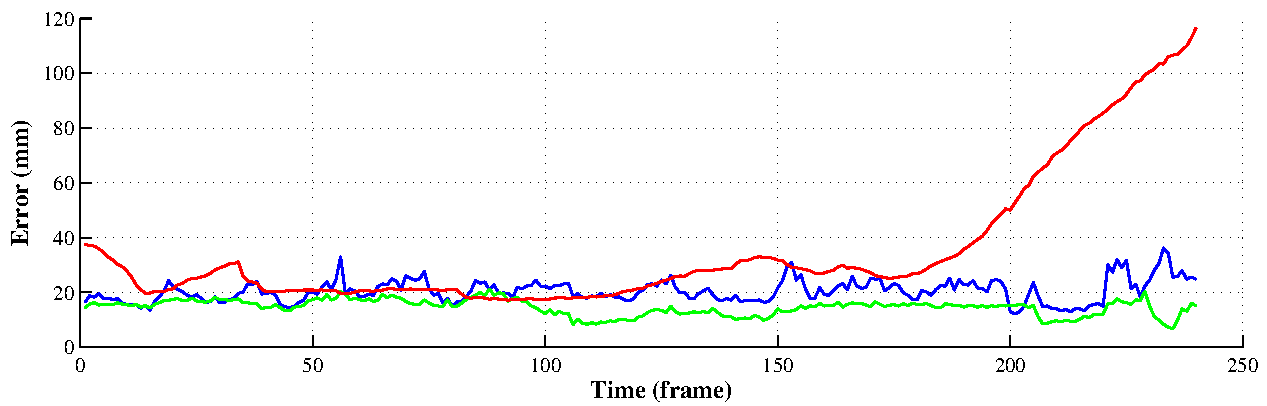
\includegraphics[width=0.33\linewidth]{fig/hand/sq2_avg.pdf} 
%	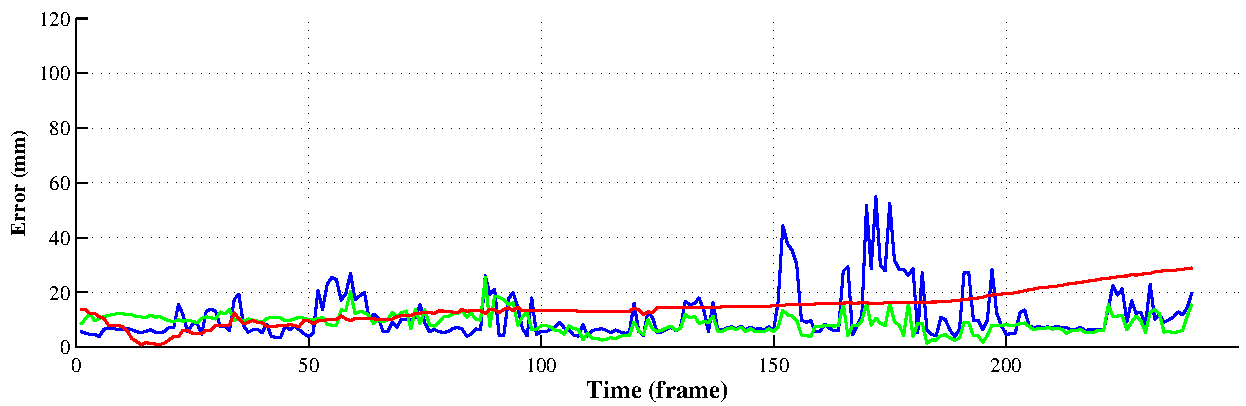
\includegraphics[width=0.31\linewidth]{fig/hand/sq2_palm.pdf}
%	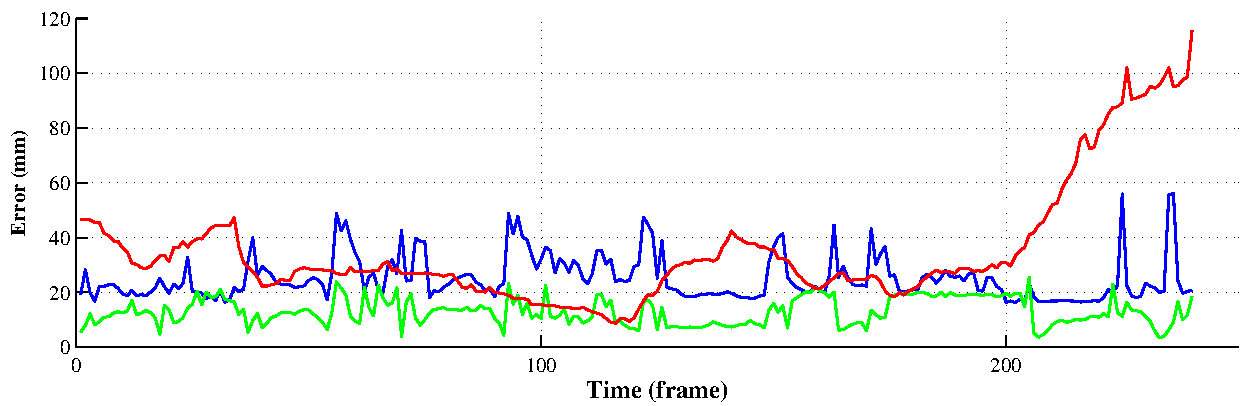
\includegraphics[width=0.31\linewidth]{fig/hand/sq2_tip.pdf} 
%	\caption{Joint localisation errors of the multiview testing squences.}
%	\label{fig/hand/multiquant}
%\end{figure}

\begin{figure}[ht]
	\centering
	\subcaptionbox{Test sequence $B$ (Average error)\label{fig/hand/multiquanta}}{
		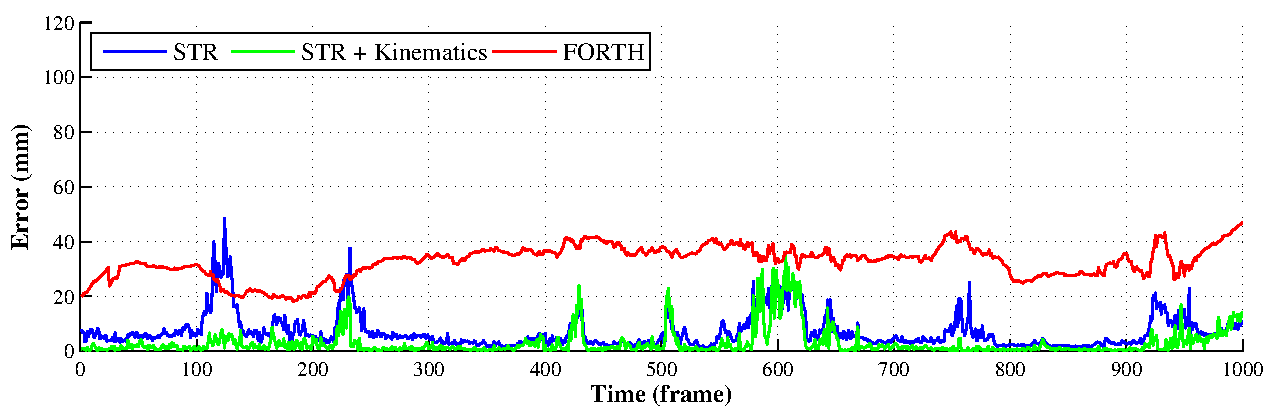
\includegraphics[width=0.48\linewidth]{fig/hand/sq1_avg.pdf}
	}
	\subcaptionbox{Test sequence $C$ (Average error)\label{fig/hand/multiquantb}}{
		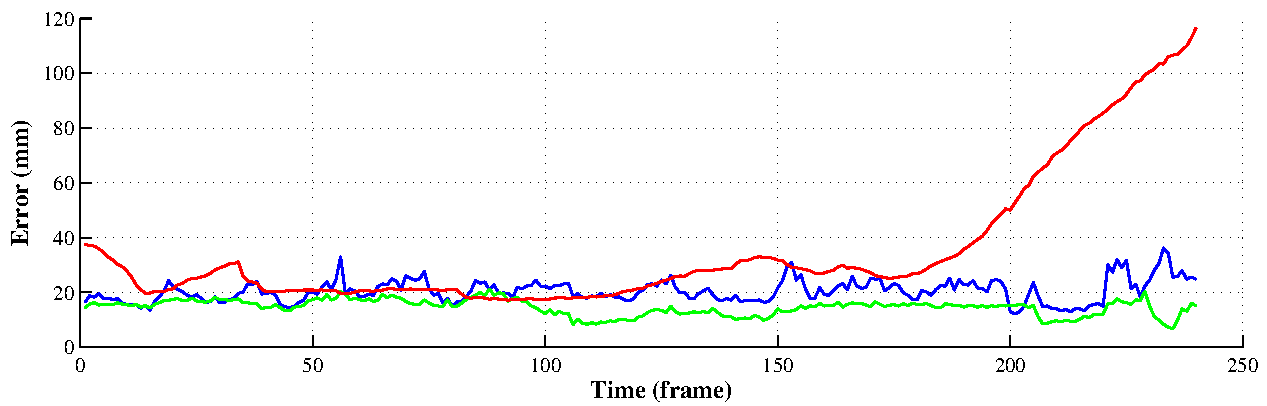
\includegraphics[width=0.48\linewidth]{fig/hand/sq2_avg.pdf}
	}\\
	\subcaptionbox{Test sequence $B$ (Palm)\label{fig/hand/multiquantc}}{
		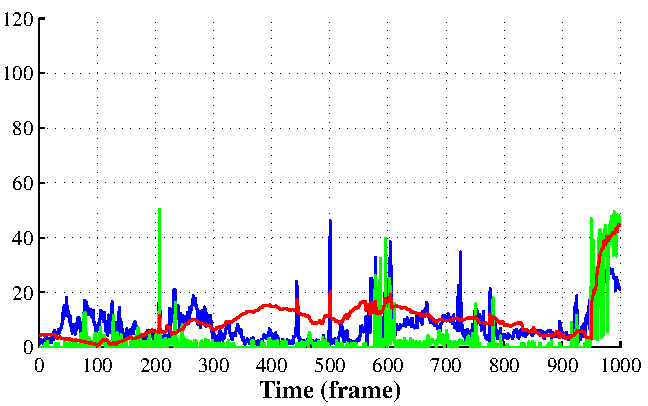
\includegraphics[width=0.48\linewidth]{fig/hand/sq1_palm.pdf}
	}
	\subcaptionbox{Test sequence $C$ (Palm)\label{fig/hand/multiquantd}}{
		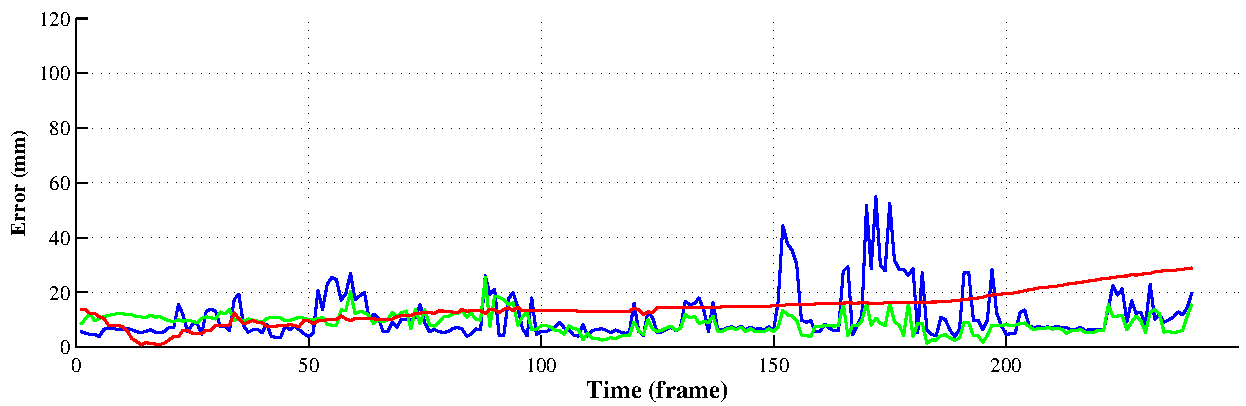
\includegraphics[width=0.48\linewidth]{fig/hand/sq2_palm.pdf}
	}\\
	\subcaptionbox{Test sequence $B$ (Index finger tip)\label{fig/hand/multiquante}}{
		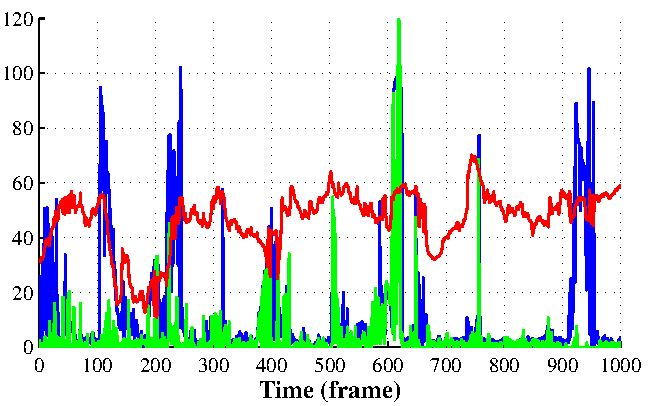
\includegraphics[width=0.48\linewidth]{fig/hand/sq1_tip.pdf}
	}
	\subcaptionbox{Test sequence $C$ (Index finger tip)\label{fig/hand/multiquantf}}{
		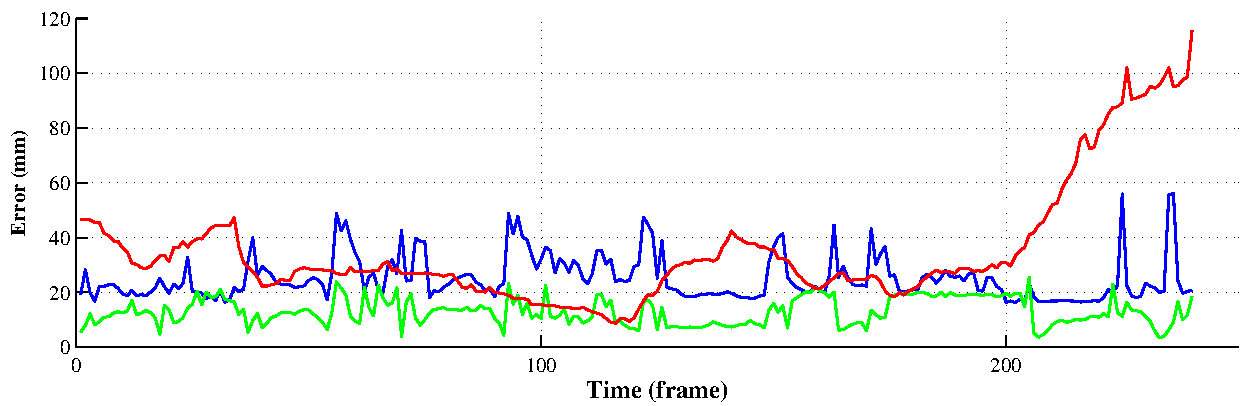
\includegraphics[width=0.48\linewidth]{fig/hand/sq2_tip.pdf}
	}
	\caption{Quantitative results of the multi-view experiment.}
	\label{fig/hand/multiquant}
\end{figure}

% 3 x 4 or 4 x 4 image array (RGB, Depth, Ours, FORTH), I expect half a page  
% show two similar poses with similar viewpoints 
% show a pose with heavy occlusion 
% shows FORTH gives large error when it loses track 
\begin{figure}
	\centering
	\begin{tabular}{@{}cc@{}c@{}c@{}c@{}c@{}}
		\textbf{Frame} & \textbf{RGB} & \textbf{Depth} & \textbf{FORTH} & \textbf{Classification} & \textbf{3D Pose} \\ 
		\hline 
		\multicolumn{6}{c}{\textbf{Testing hand sequence $B$}} \\ 
		\hline 
		\raisebox{1.3cm}{\parbox{2cm}{\centering (a)\\Frame 303}} & 
		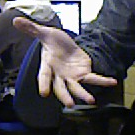
\includegraphics[width=2.35cm]{fig/hand/qual/rgb/image_0303.png} &
		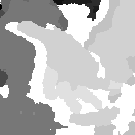
\includegraphics[width=2.35cm]{fig/hand/qual/depth/image_0303.png} &
		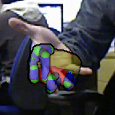
\includegraphics[width=2.35cm]{fig/hand/qual/forth/image_0303.png} &
		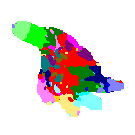
\includegraphics[width=2.35cm]{fig/hand/qual/class/class-303.png} &
		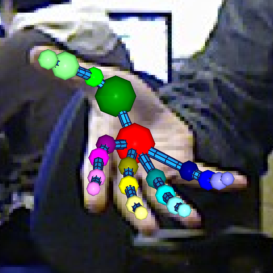
\includegraphics[width=2.35cm]{fig/hand/qual/vote/image_0303.png}
		\phantomsubcaption\label{fig/hand/multi1} \\
		\raisebox{1cm}{\parbox{2cm}{\centering (b)\\Frame 520}} & 
		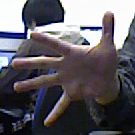
\includegraphics[width=2.35cm]{fig/hand/qual/rgb/image_0520.png} &
		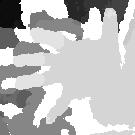
\includegraphics[width=2.35cm]{fig/hand/qual/depth/image_0520.png} &
		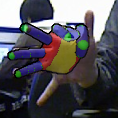
\includegraphics[width=2.35cm]{fig/hand/qual/forth/image_0520.png} &
		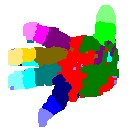
\includegraphics[width=2.35cm]{fig/hand/qual/class/class-520.png} &
		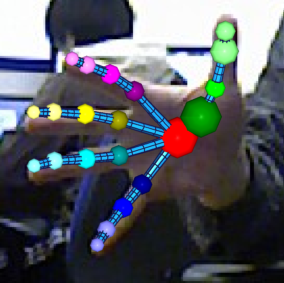
\includegraphics[width=2.35cm]{fig/hand/qual/vote/image_0520.png}
		\phantomsubcaption\label{fig/hand/multi2} \\
		\raisebox{1cm}{\parbox{2cm}{\centering (c)\\Frame 825}} & 
		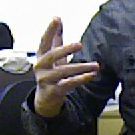
\includegraphics[width=2.35cm]{fig/hand/qual/rgb/image_0825.png} &
		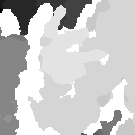
\includegraphics[width=2.35cm]{fig/hand/qual/depth/image_0825.png} &
		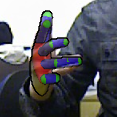
\includegraphics[width=2.35cm]{fig/hand/qual/forth/image_0825.png} &
		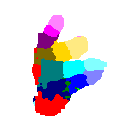
\includegraphics[width=2.35cm]{fig/hand/qual/class/class-825.png} &
		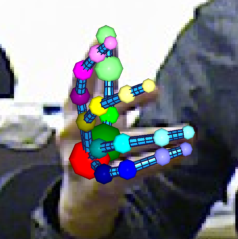
\includegraphics[width=2.35cm]{fig/hand/qual/vote/image_0825.png}
		\phantomsubcaption\label{fig/hand/multi3} \\
		\raisebox{1cm}{\parbox{2cm}{\centering (d)\\Frame 946}} & 
		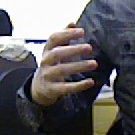
\includegraphics[width=2.35cm]{fig/hand/qual/rgb/image_0946.png} &
		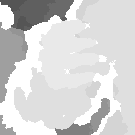
\includegraphics[width=2.35cm]{fig/hand/qual/depth/image_0946.png} &
		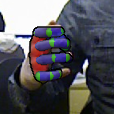
\includegraphics[width=2.35cm]{fig/hand/qual/forth/image_0946.png} &
		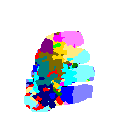
\includegraphics[width=2.35cm]{fig/hand/qual/class/class-946.png} &
		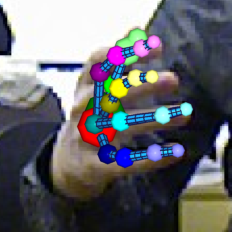
\includegraphics[width=2.35cm]{fig/hand/qual/vote/image_0946.png}
		\phantomsubcaption\label{fig/hand/multi4} \\
		\raisebox{1cm}{\parbox{2cm}{\centering (e)\\Frame 996}} & 
		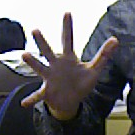
\includegraphics[width=2.35cm]{fig/hand/qual/rgb/image_0996.png} &
		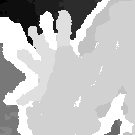
\includegraphics[width=2.35cm]{fig/hand/qual/depth/image_0996.png} &
		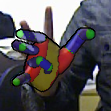
\includegraphics[width=2.35cm]{fig/hand/qual/forth/image_0996.png} &
		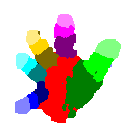
\includegraphics[width=2.35cm]{fig/hand/qual/class/class-996.png} &
		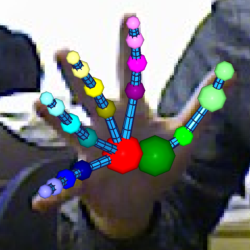
\includegraphics[width=2.35cm]{fig/hand/qual/vote/image_0996.png}
		\phantomsubcaption\label{fig/hand/multi5} \\ 
		\hline 
		\multicolumn{6}{c}{\textbf{Testing hand sequence $C$}} \\ 
		\hline 
		\raisebox{1cm}{\parbox{2cm}{\centering (f)\\Frame 198}} &
		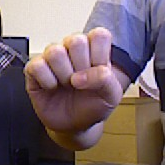
\includegraphics[width=2.35cm]{fig/hand/qual/rgb/image_0198.png} &
		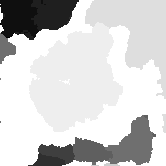
\includegraphics[width=2.35cm]{fig/hand/qual/depth/image_0198.png} &
		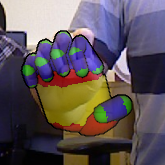
\includegraphics[width=2.35cm]{fig/hand/qual/forth/image_0198.png} &
		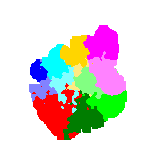
\includegraphics[width=2.35cm]{fig/hand/qual/class/class-198.png} &
		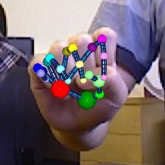
\includegraphics[width=2.35cm]{fig/hand/qual/vote/image_0198.png} 
		\phantomsubcaption\label{fig/hand/multi6} \\
		\raisebox{1cm}{\parbox{2cm}{\centering (g)\\Frame 440}} & 
		\includegraphics[width=2.35cm]{fig/hand/qual/rgb/image_0440.png} &
		\includegraphics[width=2.35cm]{fig/hand/qual/depth/image_0440.png} &
		\includegraphics[width=2.35cm]{fig/hand/qual/forth/image_0440.png} &
		\includegraphics[width=2.35cm]{fig/hand/qual/class/class-440.png} &
		\includegraphics[width=2.35cm]{fig/hand/qual/vote/image_0440.png} 
		\phantomsubcaption\label{fig/hand/multi7} \\
	\end{tabular}
	\caption{\textbf{Qualitative experimental results of the multi-view experiment.} For each row, from left to right: RGB image, depth image, hand pose from FORTH, joint labels from the proposed method, final hand pose output of the proposed method.}
	\label{fig/hand/multiqual}
\end{figure} 
 

\section{Discussion}

This chapter presents the first semi-supervised transductive approach for articulated hand pose estimation.  
Despite its similarity with body pose estimation, techniques for articulated hand pose is still far from mature, primarily due to the unique issues of occlusion and noise issues in hand pose data. 
On the other hand, the discrepancies between realistic and synthetic data also undermine the performances of state-of-the-arts. 

Addressing the aforementioned issues, we propose a novel discriminative approach, \STR\ forest, to estimate hand articulations using both realistic and synthetic data. With transductive learning, the \STR\ forest recognises a wide range of poses from a small number of labelled realistic data. Semi-supervised learning is applied to fully utilise the sparsely labelled realistic dataset. Besides, we also present a data-driven pseudo-kinematic technique, as means to improve the estimation accuracy of occluded and noisy hand poses. 

The proposed approach is evaluated with respect to different challenging environments.    
From the quantitative and qualitative analyses conducted, our method has demonstrated promising results in estimating articulated hand poses from noisy and strongly occluded data.  
It also attains superior performances and speed compared with state-of-the-art.  
